\section{Implementation}
\begin{frame}{Implementation}
    \begin{itemize}
        \item Data Collection
        \item Data Augmentation
        \item Classification Model
        \item Virtual Environment
    \end{itemize}
\end{frame}

\subsection*{Data Collection}
\begin{frame}{Data Collection}
    \begin{minipage}[c]{.6\textwidth}
        \begin{itemize}
            \item Datasets: Physionet, Weibo, BCI Competition IV
            \item Channels: 58
            \item Frequency Bandpass Filter: 0.5~\textemdash{}~40 Hz
            \item Start-End Window Time: 0.0~\textemdash{}~0.5 s
            \item Sampling Frequency: 128 Hz
        \end{itemize}
    \end{minipage}
    \begin{minipage}[c]{.39\textwidth}
        \begin{figure}[!htbp]
            \centering
            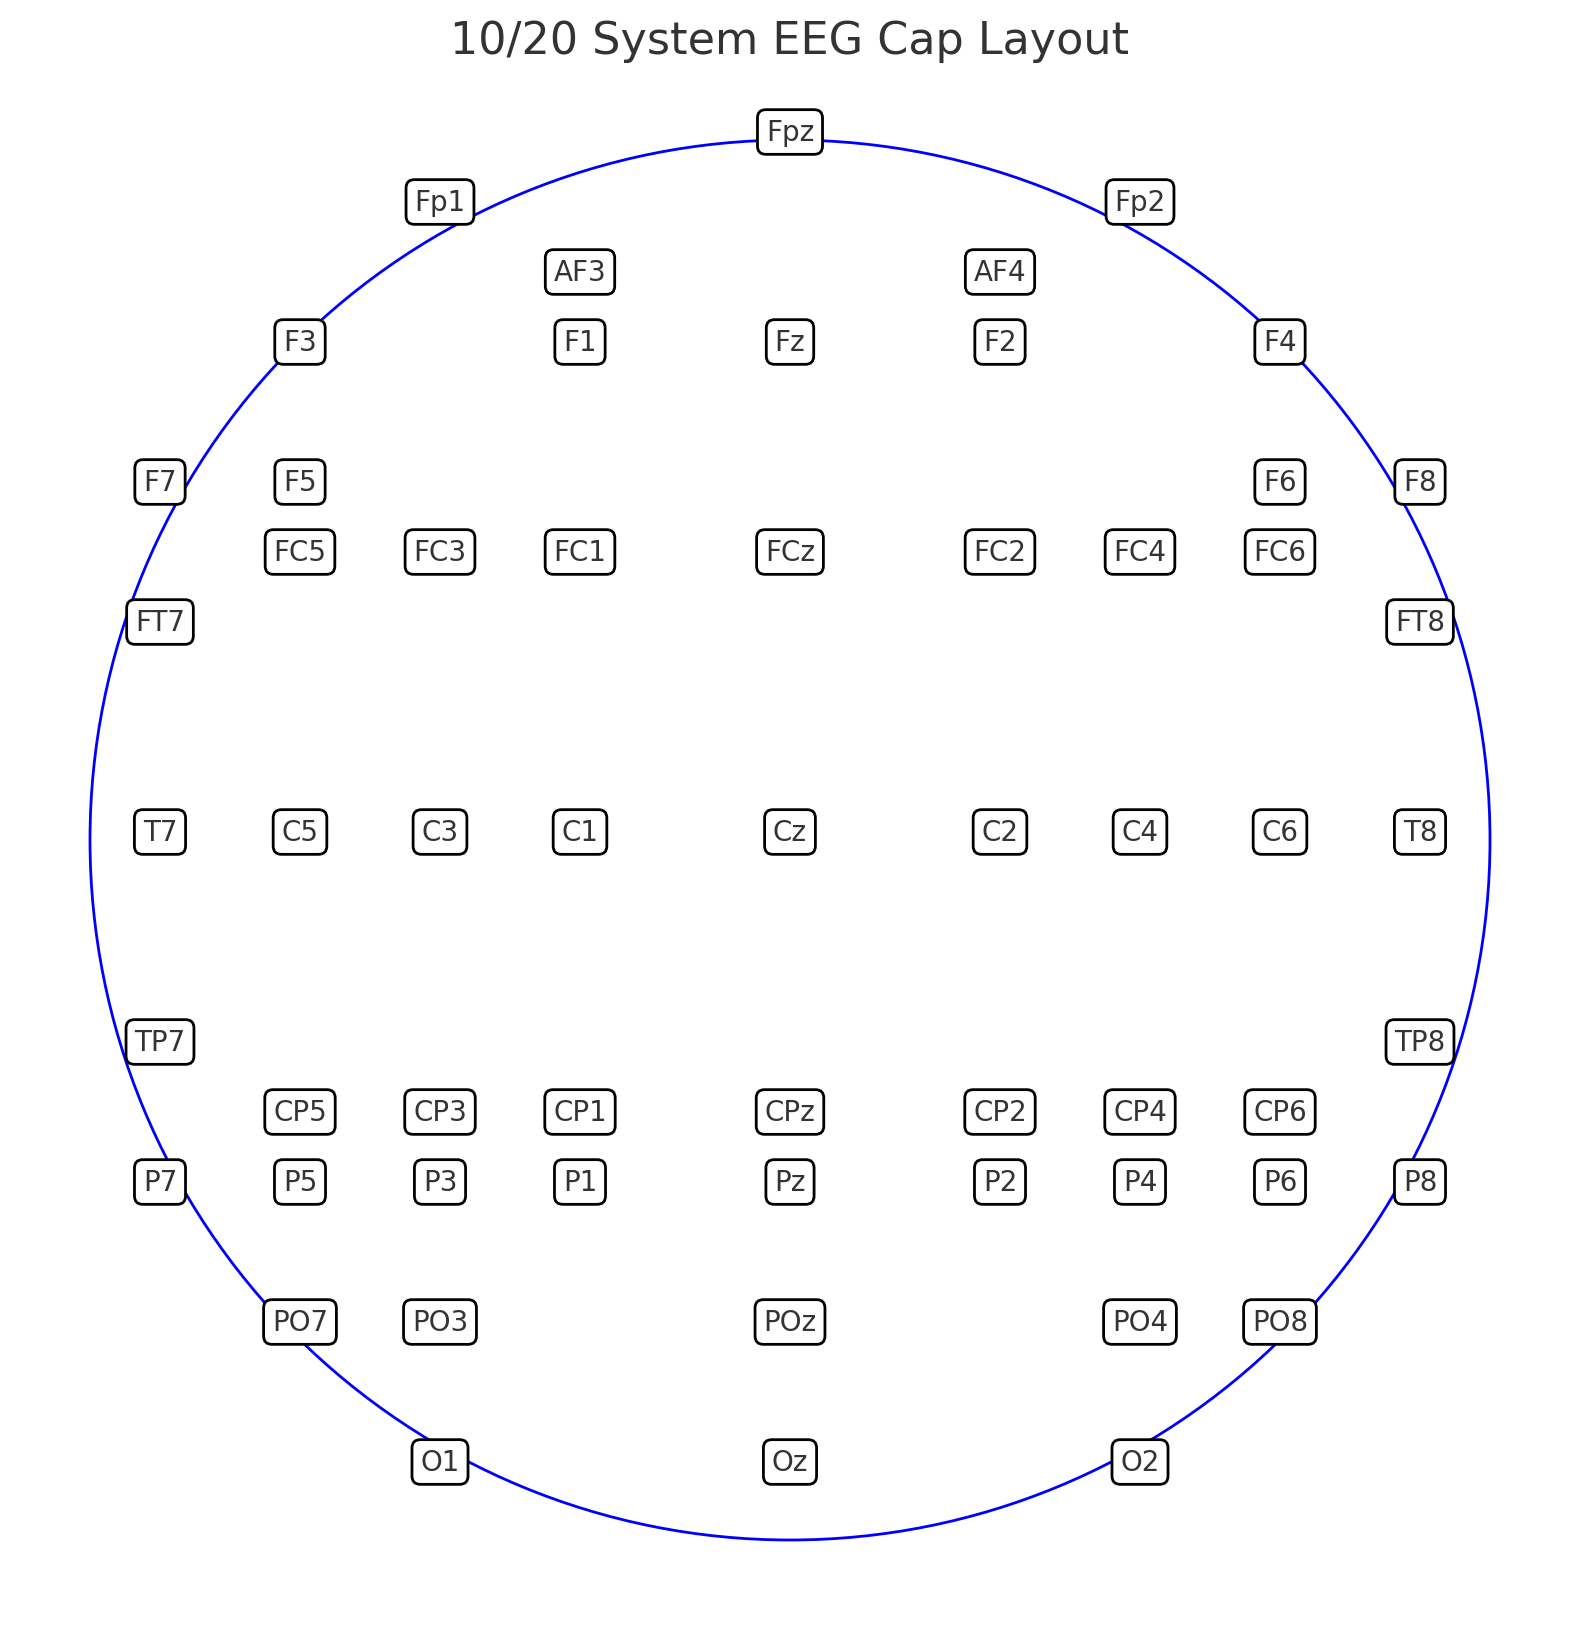
\includegraphics[width=0.5\textwidth]{figures/Methodology/thesis_eeg_cap}
        \end{figure}
    \end{minipage}
\end{frame}

\subsection*{Data Augmentation}
\begin{frame}{Data Augmentation}
    \begin{itemize}
        \item Stochastic Noise Injection
        \item Generative Adversarial Networks (GANs)
    \end{itemize}
\end{frame}
\begin{frame}{Data Augmentation \textemdash{} Noise Injection}
    \begin{itemize}
        \item Reduced Dataset size
        \item Gaussian Noise
        \begin{itemize}
            \item Mean: 0.0
            \item Standard Deviation: 1.0
        \end{itemize}
    \end{itemize}
\end{frame}
\begin{frame}{Data Augmentation \textemdash{} GANs}
    \begin{minipage}[c]{.6\textwidth}
        \begin{itemize}
            \item Loss Function: Binary Cross-Entropy
            \item Optimizer: Adam
            \item Learning Rate: 0.0002
            \item Train Epochs: 100 epochs, with changing number of steps
        \end{itemize}
    \end{minipage}
    \begin{minipage}[c]{.39\textwidth}
        \begin{figure}[!htbp]
            \centering
            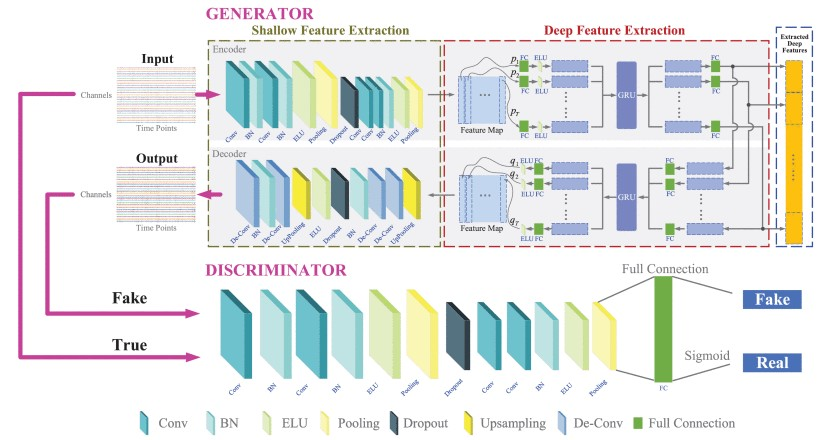
\includegraphics[width=\textwidth]{figures/Methodology/GAN}
        \end{figure}
    \end{minipage}
\end{frame}

\subsection*{Classification Model}
\begin{frame}{Classification Model}
    \begin{itemize}
        \item Long Short-Term Memory (LSTM)
        \item Attention Mechanism
    \end{itemize}
\end{frame}
\begin{frame}{Classification Model \textemdash{} LSTM}
    % todo: fix values
    \begin{minipage}[c]{.6\textwidth}
        \begin{itemize}
            \item Hidden Units: 128
            \item Activation Function: Sigmoid
            \item Optimizer: Adam
            \item Learning Rate: 0.001
            \item Loss Function: Binary Cross-Entropy
        \end{itemize}
    \end{minipage}
    \begin{minipage}[c]{.39\textwidth}
        \begin{figure}[!htbp]
            \centering
            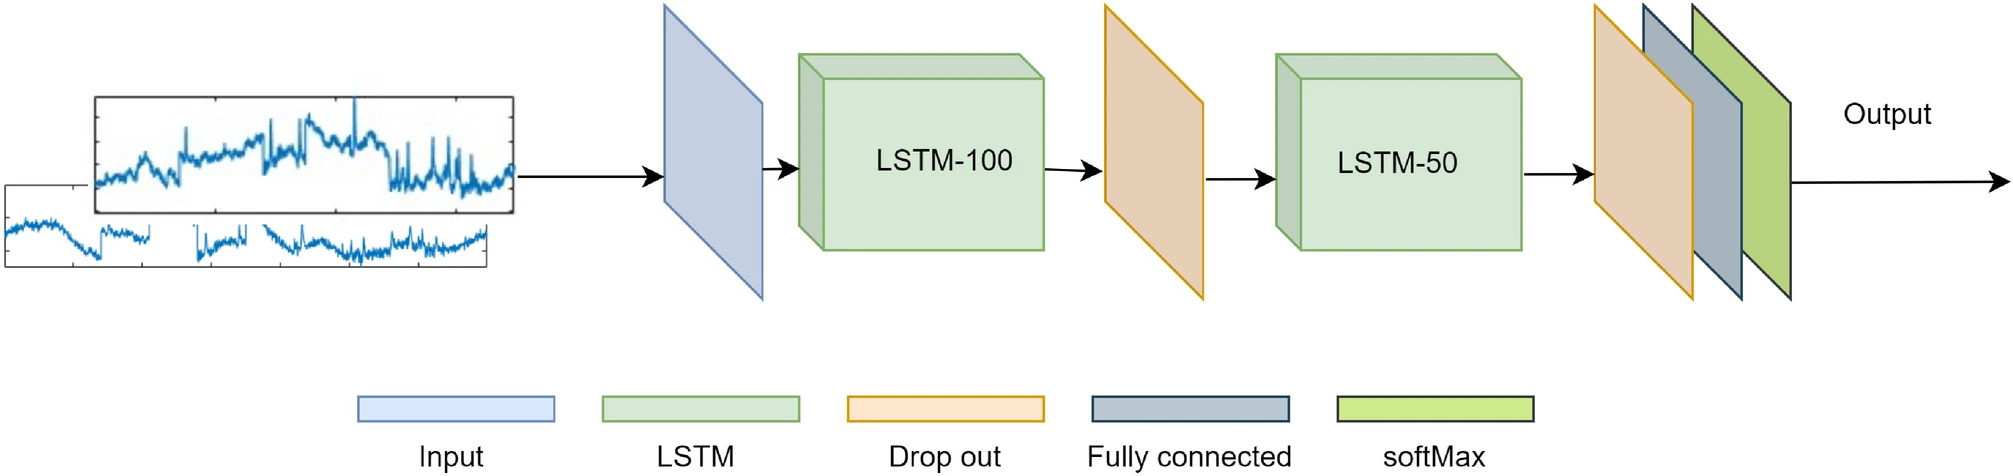
\includegraphics[width=\textwidth]{figures/Methodology/LSTM}
        \end{figure}
    \end{minipage}
\end{frame}
\begin{frame}{Classification Model \textemdash{} Attention Mechanism}
    % todo: fix values
    \begin{minipage}[c]{.6\textwidth}
        \begin{itemize}
            \item Hidden Units: 128
            \item Activation Function: Sigmoid
            \item Optimizer: Adam
            \item Learning Rate: 0.001
            \item Loss Function: Binary Cross-Entropy
        \end{itemize}
    \end{minipage}
    \begin{minipage}[c]{.39\textwidth}
        \begin{figure}[!htbp]
            \centering
            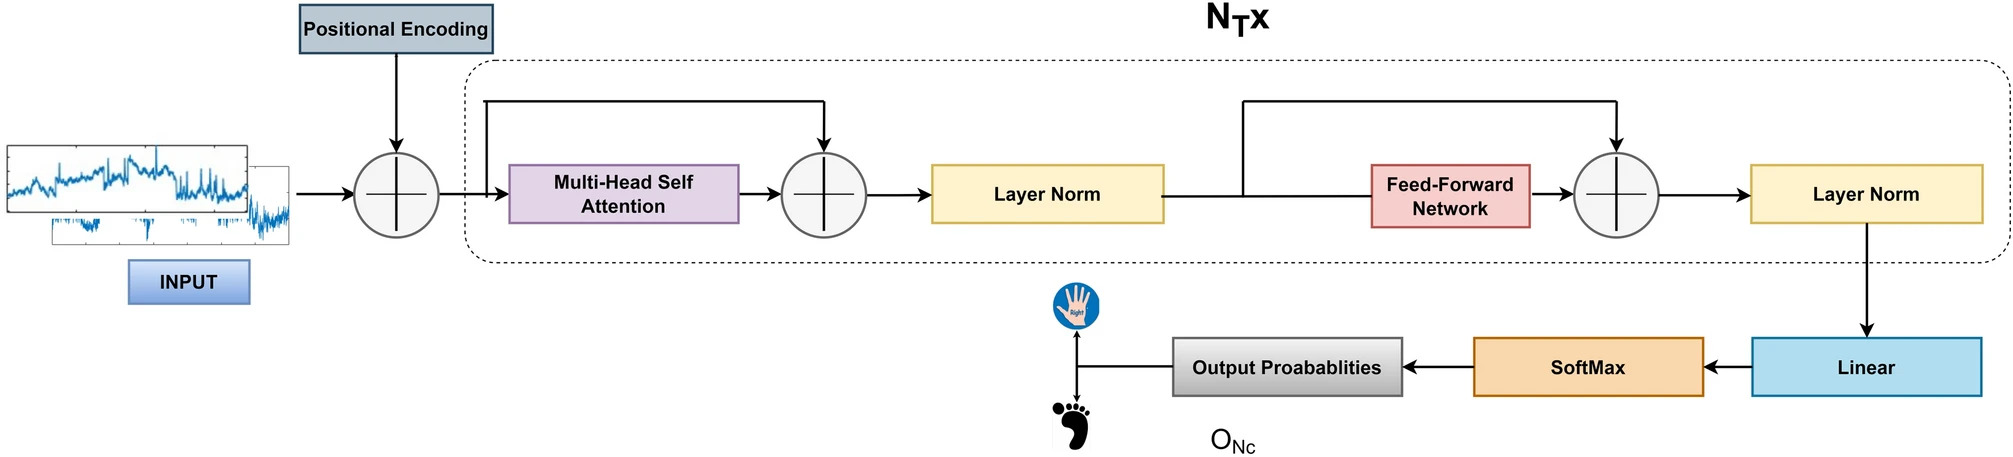
\includegraphics[width=\textwidth]{figures/Methodology/Attention}
        \end{figure}
    \end{minipage}
\end{frame}

\subsection*{Virtual Environment}
\begin{frame}{Virtual Environment}
    \begin{minipage}[c]{.6\textwidth}
        \begin{itemize}
            \item TextMeshPro
            \item Starter Assets \textemdash{} Third Person Controller
            \item Native Websocket $\xrightarrow{}$ Open source library
            \item Unity AI Navigation
            \item Maze Generator $\xrightarrow{}$ Free Unity Asset
        \end{itemize}
    \end{minipage}
    \begin{minipage}[c]{.39\textwidth}
        \begin{figure}[!htbp]
            \centering
            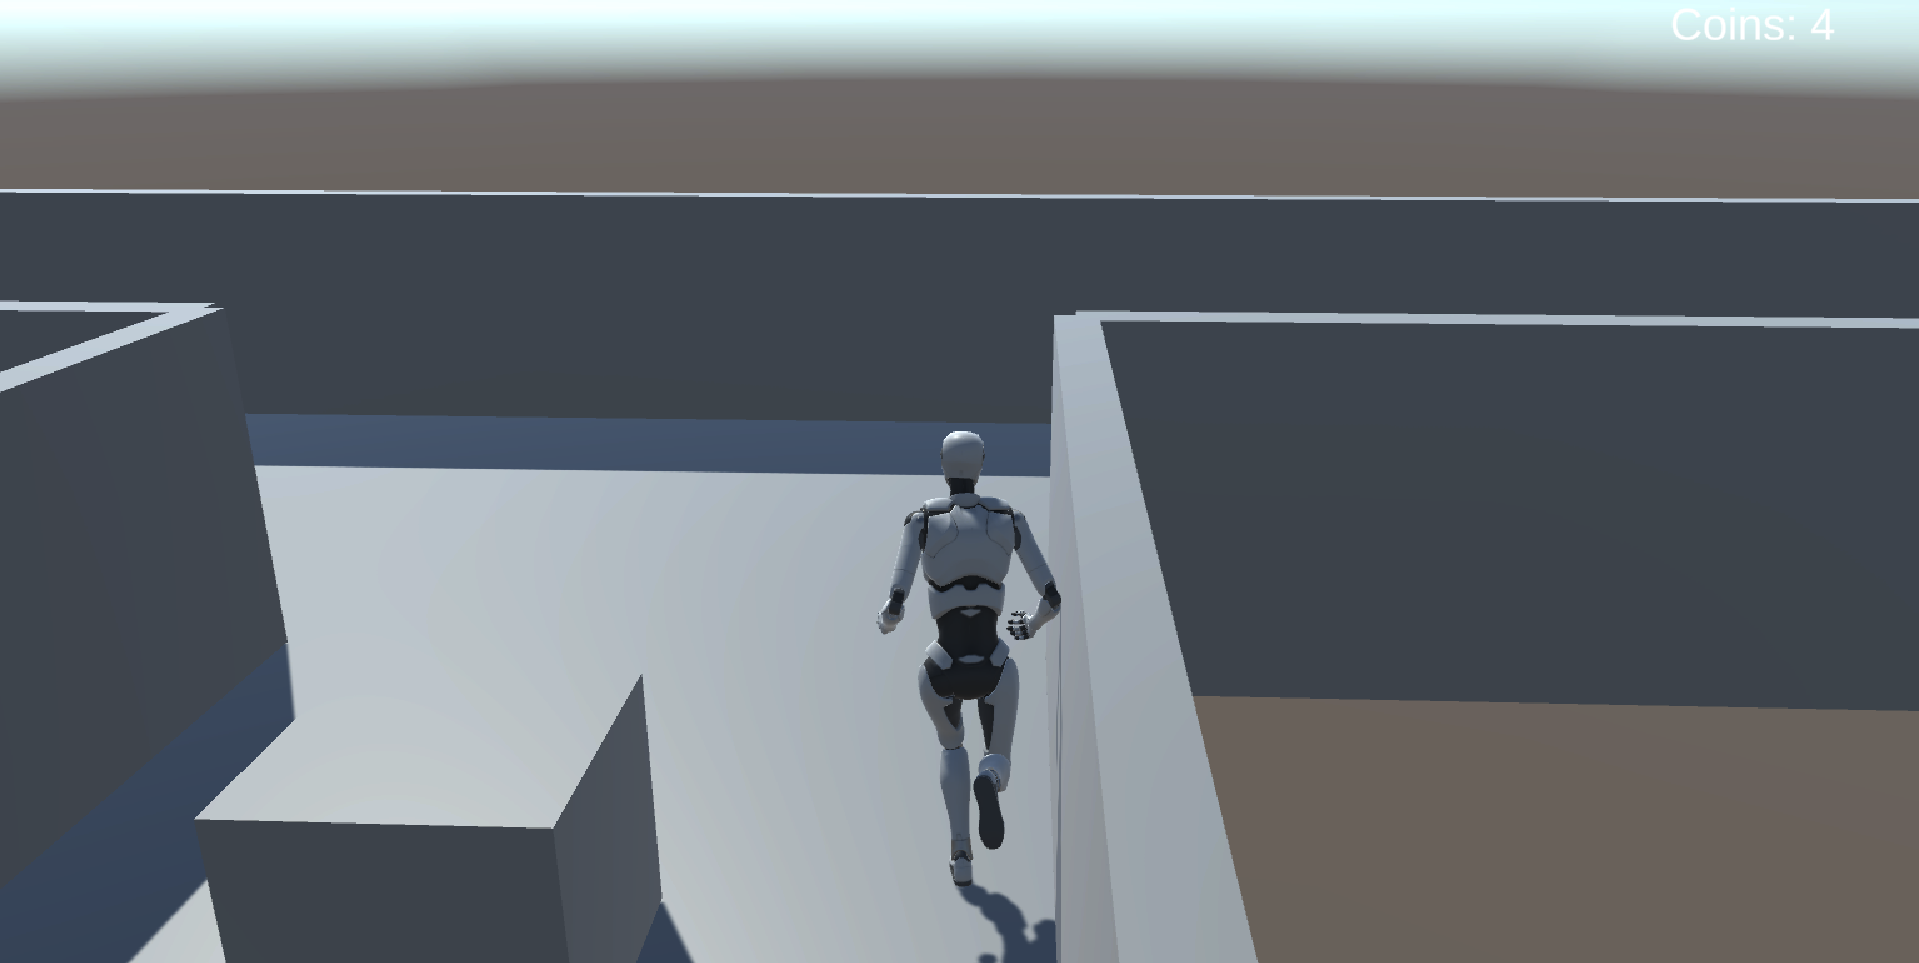
\includegraphics[width=\textwidth]{figures/Methodology/infinite_runner}
            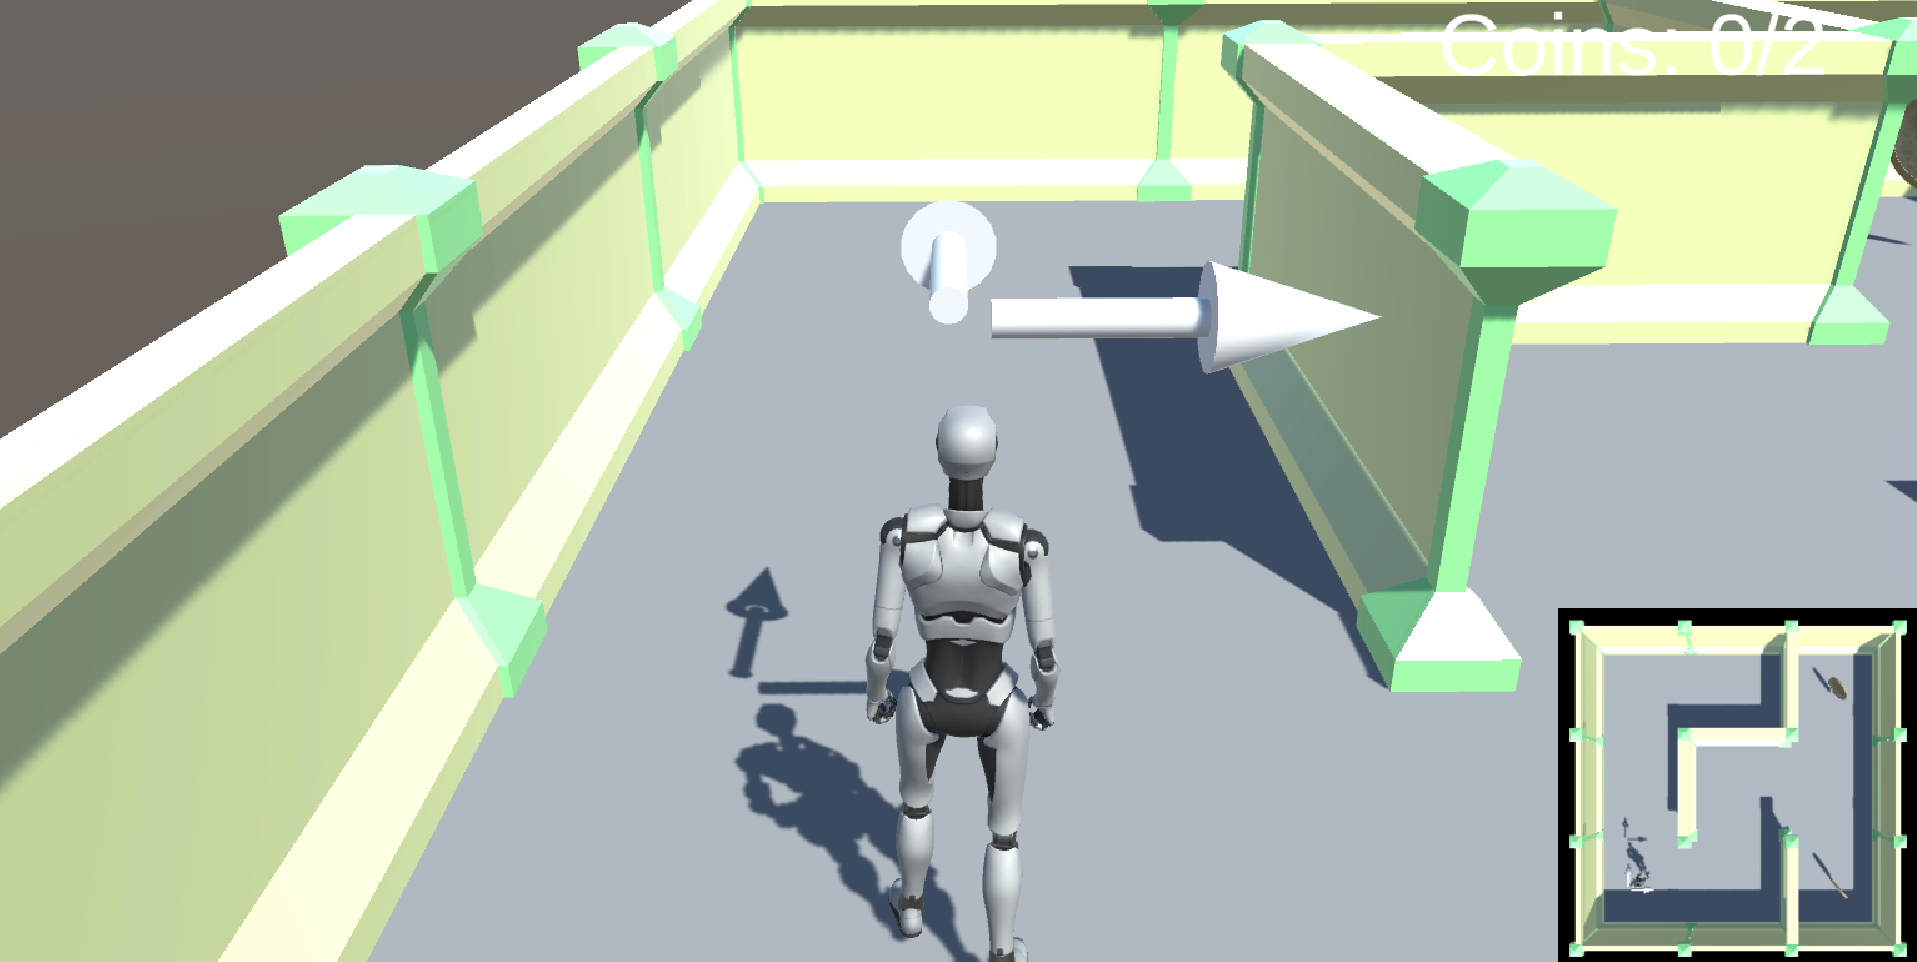
\includegraphics[width=\textwidth]{figures/Methodology/maze}
        \end{figure}
    \end{minipage}
\end{frame}
